\begin{appendices}
\section{Quellcode-Frontend}
\subsection{PureScript}
\lstinputlisting{../FROST-Frontend/src/Openspace/Engine.purs}
\lstinputlisting{../FROST-Frontend/src/Openspace/Types.purs}
\lstinputlisting{../FROST-Frontend/src/Openspace/Network/Socket.purs}
\lstinputlisting{../FROST-Frontend/src/Openspace/Ui/Render.purs}
\lstinputlisting{../FROST-Frontend/src/Openspace/Ui/Parser.purs}
\lstinputlisting{../FROST-Frontend/src/Openspace/Ui/Emitter.purs}
\lstinputlisting{../FROST-Frontend/src/Openspace/Ui/Stream.purs}
\subsection{JavaScript}
\lstinputlisting[language=Javascript]{../FROST-Frontend/static/grid.js}
\lstinputlisting[language=Javascript]{../FROST-Frontend/static/menu.js}
\lstinputlisting[language=Javascript]{../FROST-Frontend/static/topics.js}
\subsection{CSS}
\lstinputlisting[language=CSS]{../FROST-Frontend/static/main.css}
\subsection{HTML}
\lstinputlisting[language=html]{../FROST-Frontend/static/index.html}
\section{Quellcode-Backend}
\subsection{Haskell}
\lstinputlisting{../FROST-Backend/src/Foundation.hs}
\lstinputlisting{../FROST-Backend/src/Import.hs}
\lstinputlisting{../FROST-Backend/src/Main.hs}
\lstinputlisting{../FROST-Backend/src/Application/Engine.hs}
\lstinputlisting{../FROST-Backend/src/Application/Types.hs}
\lstinputlisting{../FROST-Backend/src/Application/TopicTypes.hs}
\lstinputlisting{../FROST-Backend/src/Handler/Admin.hs}
\lstinputlisting{../FROST-Backend/src/Handler/Socket.hs}
\lstinputlisting{../FROST-Backend/src/Handler/Snapshot.hs}

\section{Build-Scripts}
\subsection{Frontend}
\lstinputlisting[language=bash]{../FROST-Frontend/build.sh}
\subsection{Backend}
\lstinputlisting[language=bash]{../FROST-Backend/build.sh}

\section{Screenshots}
\subsection{Desktop-Version}
\begin{sidewaysfigure}
    \centering
    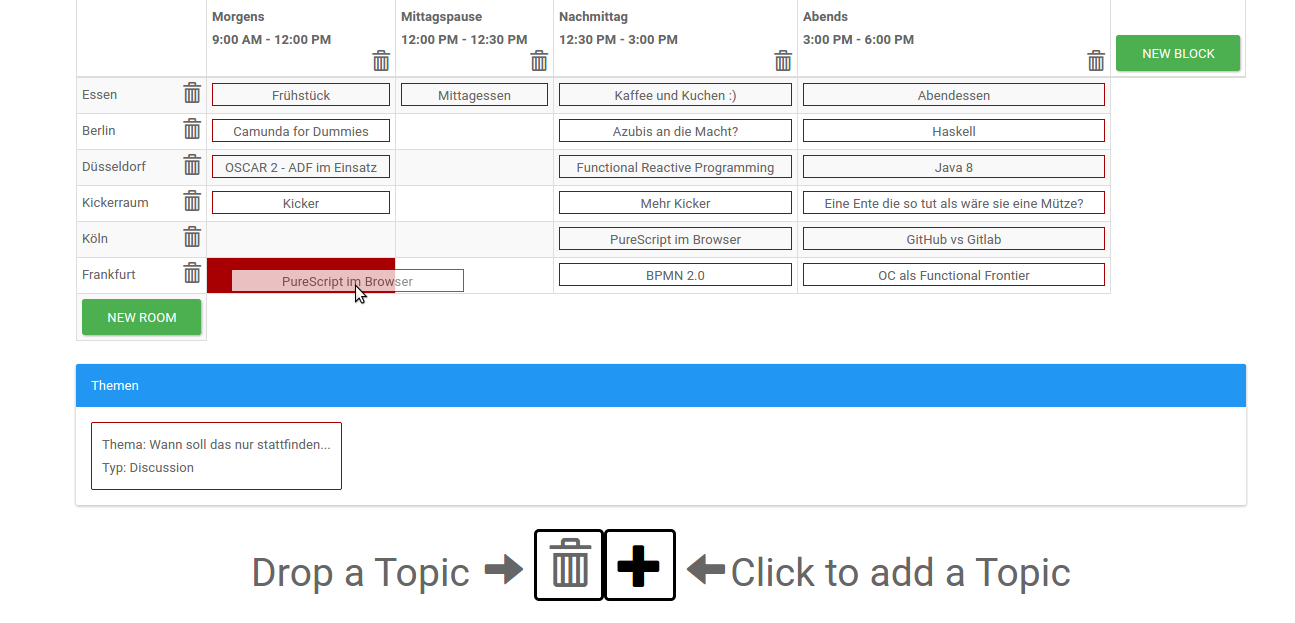
\includegraphics[scale=0.5]{img/desktop_screenshot.png}
    \caption{Screenshot Desktop}
    %\label{fig:awesome_image}
\end{sidewaysfigure}

\begin{sidewaysfigure}
    \centering
    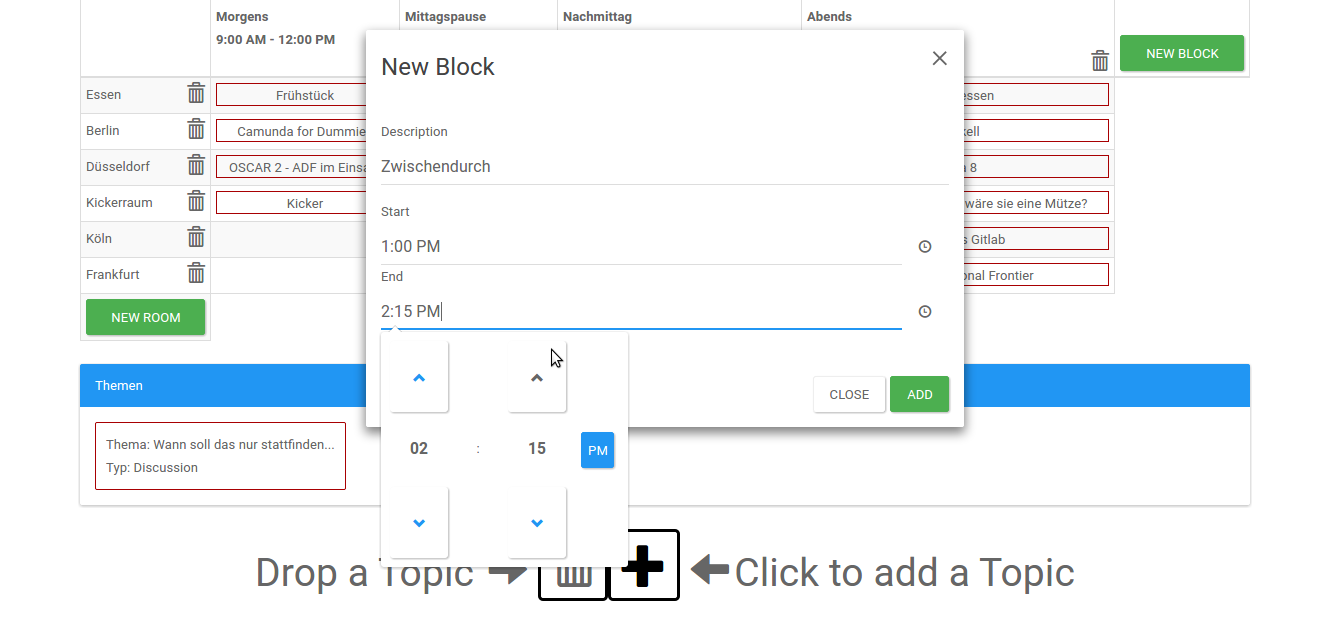
\includegraphics[scale=0.5]{img/neuer_block_screenshot.png}
    \caption{Screenshot Neuer Block}
    %\label{fig:awesome_image}
\end{sidewaysfigure}

\begin{sidewaysfigure}
    \centering
    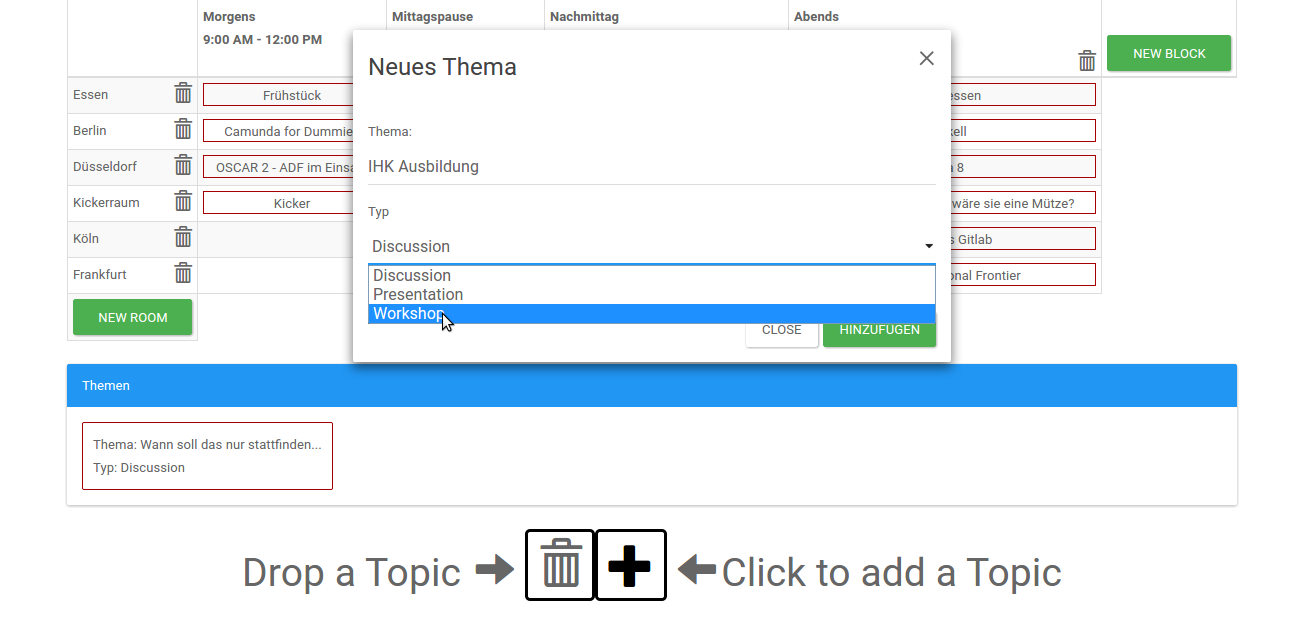
\includegraphics[scale=0.5]{img/neues_thema_screenshot.png}
    \caption{Screenshot Neues Thema}
    %\label{fig:awesome_image}
\end{sidewaysfigure}
\clearpage
\subsection{Mobile-Version}
\begin{figure}[h]
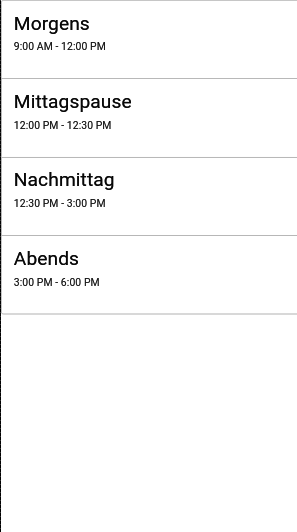
\includegraphics[scale=0.8]{img/mobile_view.png}
\caption{Screenshot Mobile Ansicht}
\end{figure}
\begin{figure}[h]
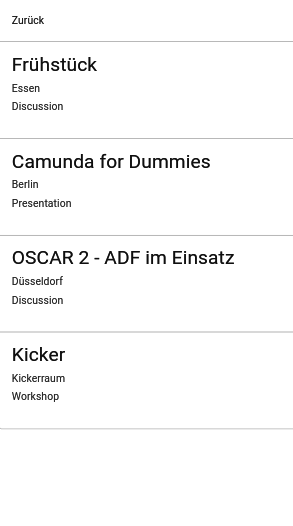
\includegraphics[scale=0.8]{img/mobile_inner_screenshot.png}
\caption{Screenshot Mobile Detailansicht}
\end{figure}
\end{appendices}

%%% Local Variables:
%%% mode: latex
%%% TeX-master: "../Doku"
%%% End:
